\documentclass[aspectratio=169]{beamer}
\usepackage[utf8]{inputenc}

\usetheme{Madrid}
\usecolortheme{default}

%------------------------------------------------------------
%This block of code defines the information to appear in the
%Title page
\title{Introduction to Neural Networks}  
\subtitle{Design of experiment (DOE)} 
\author[J.I. Vasquez]{\textbf{Juan Irving Vásquez} \\jivg.org}
\date{\today \copyright}
\institute[jivg.org]{Centro de Innovación y Desarrollo Tecnológico en Cómputo \\ Instituto Politécnico Nacional}
% logo of my university
\titlegraphic{
\includegraphics[height=1.2cm]{ipn-cidetec.png}\hspace{0.1cm}
\includegraphics[height=1.2cm]{escudoESCOM}}


%End of title page configuration block
%------------------------------------------------------------


%------------------------------------------------------------
%The next block of commands puts the table of contents at the 
%beginning of each section and highlights the current section:

\AtBeginSection[]
{
  \begin{frame}
    \frametitle{Table of Contents}
    \tableofcontents[currentsection]
  \end{frame}
}
%------------------------------------------------------------


\begin{document}

%The next statement creates the title page.
\frame{\titlepage}



%---------------------------------------------------------
%This block of code is for the table of contents after
%the title page
\begin{frame}
\frametitle{Table of Contents}
\tableofcontents
\end{frame}
%---------------------------------------------------------

\section{Introduction}


\begin{frame}{The problem}
    
\begin{columns}
\begin{column}{0.45\textwidth}
    \begin{itemize}
    	\item Training neural networks can be tricky
        \item This applies to Research and Learning
        \item Experimentation can lead to nowhere
    \end{itemize}
\end{column}
\begin{column}{0.45\textwidth}  %%<--- here
    \begin{center}
     
\includegraphics[width=\textwidth]{phd-1.jpg}
     \end{center}
\end{column}
\end{columns}    
\end{frame}


\begin{frame}{The solution}
\begin{columns}
\begin{column}{0.45\textwidth}
    \begin{itemize}
        \item The wrong way
        \begin{itemize}
            \item Feelings
            \item Asking in facebook
            \item Asking chatgpt?
        \end{itemize}
        \pause
        \item The good way - decrease the uncertainty
        \begin{itemize}
            \item Experimental design
            \item Hyper-parameter optimization
        \end{itemize}
    \end{itemize}
\end{column}
\begin{column}{0.45\textwidth}  %%<--- here
    \begin{center}
     
\includegraphics[width=\textwidth]{start.jpg}
     \end{center}
\end{column}
\end{columns}
\end{frame}


\section{Design of experiment}


\begin{frame}
\frametitle{Design of experiment}
\framesubtitle{Terminology}
    \begin{description}
    \item [Subject] \hfill \\ Task and dataset (Classification, detection, etc)
    \item [Factor] \hfill \\ Controlled independent variable (Hyper-parameter, architecture, ...)
    \item [Treatment] \hfill \\ Set of factors applied to an experimental unit (Trained architecture)
    \item [Experimental unit] \hfill \\ Single training (Training with validation)
    \item [Experiment] \hfill \\ Record of treatments (Trained netwokds) applied to a set of subjects (tasks).
    \end{description}
\end{frame}

\begin{frame}
\frametitle{Design of experiments}
\framesubtitle{Principles}
    \begin{description}
    \item [Randomization] Process of assigning treatments to experimental units. In DL subjects can receive multiple treatments.
    \item [Statistical replication] Avoid measurement uncertainty. Replicate experiments that use random variables.
%    \item [Blocking] Grouping experimental units to estimate particular sources of variation (group by datasets).
    \item [Orthogonality] The effects of different factors and interactions can be estimated in the model separately. It usually does not happen in training.
    \item [Full-factorial experiment] All possible combinations of the levels across all the factors are applied to the experimental units. Usually it is the followed in DL.
    \end{description}
\end{frame}

\begin{frame}{Full-factorial experiment}
\framesubtitle{Design space}
\begin{figure}
    \centering
    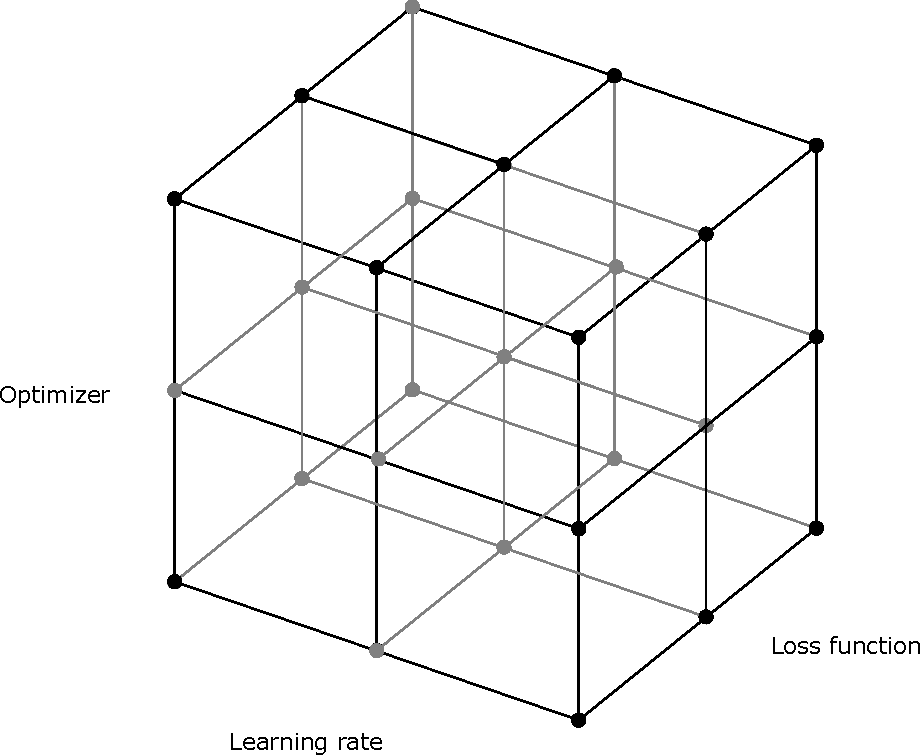
\includegraphics[height=0.65\textheight]{full factor.pdf}
    \caption{Full factorial experiment presented on a hypercube in the k-dimensional design space.}
    \label{fig:my_label}
\end{figure}
\end{frame}

\begin{frame}{Full-factorial experiment}
\framesubtitle{}
    \begin{table}[]
        \centering
        \begin{table}[]
\begin{tabular}{|l|l|l|l|}
\hline
Run & Optimizer & Learning rate & Loss function \\ \hline
1   & 1         & 1             & 1             \\ \hline
2   & 1         & 1             & 2             \\ \hline
3   & 1         & 1             & 3             \\ \hline
4   & 1         & 2             & 1             \\ \hline
5   & 1         & 2             & 2             \\ \hline
\end{tabular}
\end{table}
$\vdots$
        \caption{Example of a full-factorial table.}
        \label{tab:my_label}
    \end{table}
\end{frame}



\begin{frame}{Analysis}
    \begin{columns}
\begin{column}{0.45\textwidth}
    \begin{itemize}
    \item Several analysis can be performed
    \begin{itemize}
        \item Multiple linear regression
        \item Analysis of variance
        \item etc.
    \end{itemize}
    \item Such analysis can be overwhelming
    \item Sometimes our target is only to get "good" accuracy
\end{itemize}   
\end{column}
\begin{column}{0.45\textwidth}  %%<--- here
\pause
    \begin{center}
     
\includegraphics[width=\textwidth]{okay-im-lost.jpg}
     \end{center}
\end{column}
\end{columns}
\end{frame}

\begin{frame}{Split the experimental design}
    \begin{itemize}
        \item "High level": Formal analysis between models
        \begin{itemize}
        	\item ¿Wich is the best model?
            \item The main target our of research
            \item High level threatments
            \item Neural network architectures
        \end{itemize}
        \item "Low level": NN Hyper-parameter optimization
        \begin{itemize}
        	\item How do I get the best performance for a model?
            \item Get the best set of hyperparameters
            \item It will demonstrate the capabilities of the method
        \end{itemize}
    \end{itemize}
\end{frame}

\section{Low level: Hyper-parameter optimization}

\begin{frame}{Hyper-parameter optimization}
    Successful network training depend on multiple conditions
    \begin{itemize}
        \item Even with fixed subjects and threatments: Data and architectures
        \item Some hyper-parameters: 
        \begin{itemize}
            \item Learning rate
            \item Number of epochs
            \item Initialization
            \item Optimizer
        \end{itemize}
        \item What are the best ones?
                    $$\arg \max_\theta \rho (\Phi_\theta(X_{val}),Y_{val})$$
    \end{itemize} where $\rho$ is a performance metric, such as accuracy or F1 score.
\end{frame}


\begin{frame}{Hyper-parameter optimization}
\framesubtitle{Alternatives}
    \begin{itemize}
        \item Closed search space
        \begin{itemize}
            \item Random search
            \item Grid search
        \end{itemize}
    \item Open search space
        \begin{itemize}
                \item Optimization algorithms
                \item Genetic algorithms
                \item Bayesian optimization
        \end{itemize}
    \end{itemize}
\end{frame}

\begin{frame}{Grid search vs random search}
    \begin{figure}
        \centering
        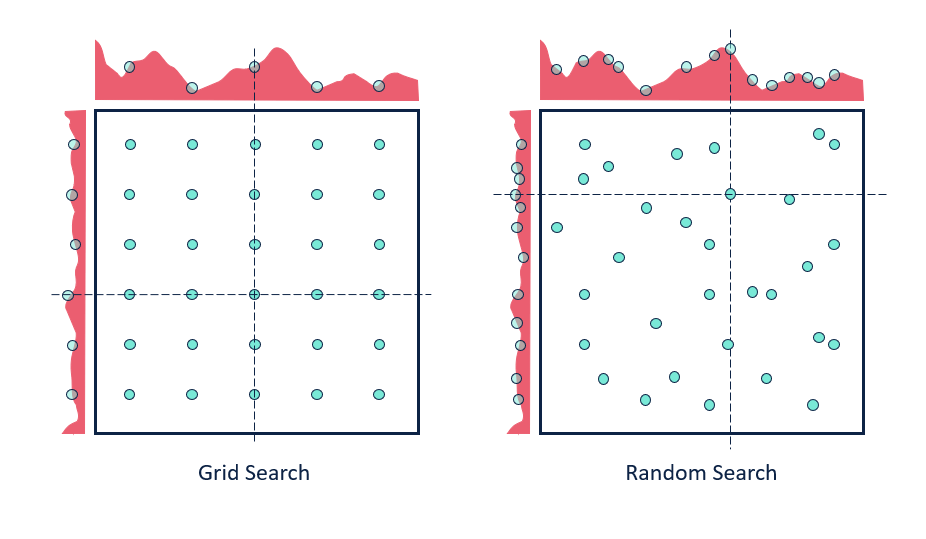
\includegraphics[height=0.8\textheight]{GridVRandom.png}
        %\caption{Caption}
        \label{fig:my_label}
    \end{figure}
\end{frame}

\section{Rule of thumb}

\begin{frame}{Rule of thumb}
\begin{columns}
	\begin{column}{0.45\textwidth}
	    \begin{enumerate}
			\item Define the problem for the individuals (data, task, metric)
			\item Define your hypothesis (VGG surpas GoogleNet in Imagenet)
			\item Define your design of experiment
			\begin{itemize}
				\item High level
				\item Low level
			\end{itemize}
			\item Launch experiments
		\end{enumerate}
	\end{column}
	\pause
	\begin{column}{0.45\textwidth}  %%<--- here
			\begin{center}
				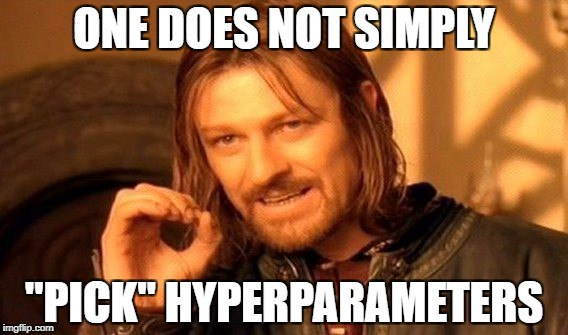
\includegraphics[width=\textwidth]{0_xMWaKlmLBHcB4AfP}
			\end{center}
	\end{column}
\end{columns}    
\end{frame}


\begin{frame}{References}
\begin{itemize}
    \item Kolosova, T., \& Berestizhevsky, S. (2020). Supervised Machine Learning: Optimization Framework and Applications with SAS and R. CRC Press.
    \item SydneyF, Hyperparameter Tuning Black Magic, \url{https://community.alteryx.com/t5/Data-Science/Hyperparameter-Tuning-Black-Magic/ba-p/449289}
\end{itemize}
\end{frame}

\end{document}
